\documentclass{templateNote}
\usepackage{tcolorbox}
\usepackage{tabularx}
\usepackage{hyperref}
\usepackage{amsmath}
\usepackage{amssymb}
\usepackage{pdflscape}
\usepackage{tikz}
\usepackage{pdfpages}
\usepackage{soul}
\usepackage{media9}
\usepackage{adjustbox}
\usepackage{enumitem}
\usepackage{pdfpages}
\usepackage{mdframed} 
\usepackage{xcolor} 
% \usepackage[spanish,es-noquoting]{babel}

\begin{document}
% \linklogoU{https://www.ubiobio.cl/w/}
\linklogoD{https://github.com/NicoGomezM}
% \imagenlogoU{img/logo-ubb-txt-face.png}
\imagenlogoD{img/logoNGMFormal_sinF.png}
\titulo{Certamen 2}
\asignatura{Investigación de Operaciones}
\autor{
    Nicolás \textsc{Gómez Morgado}
}

\portada
\margenes
\tableofcontents
\newpage




\section{Materia}
\subsection{M/M/1}
\noindent El sistema M/M/1 es un sistema de colas en el que los tiempos entre llegadas y los tiempos de servicio son variables aleatorias independientes y exponenciales. En este sistema, la tasa de llegada de clientes es $\lambda$ y la tasa de servicio es $\mu$. 

\begin{figure}[H]
    \centering
    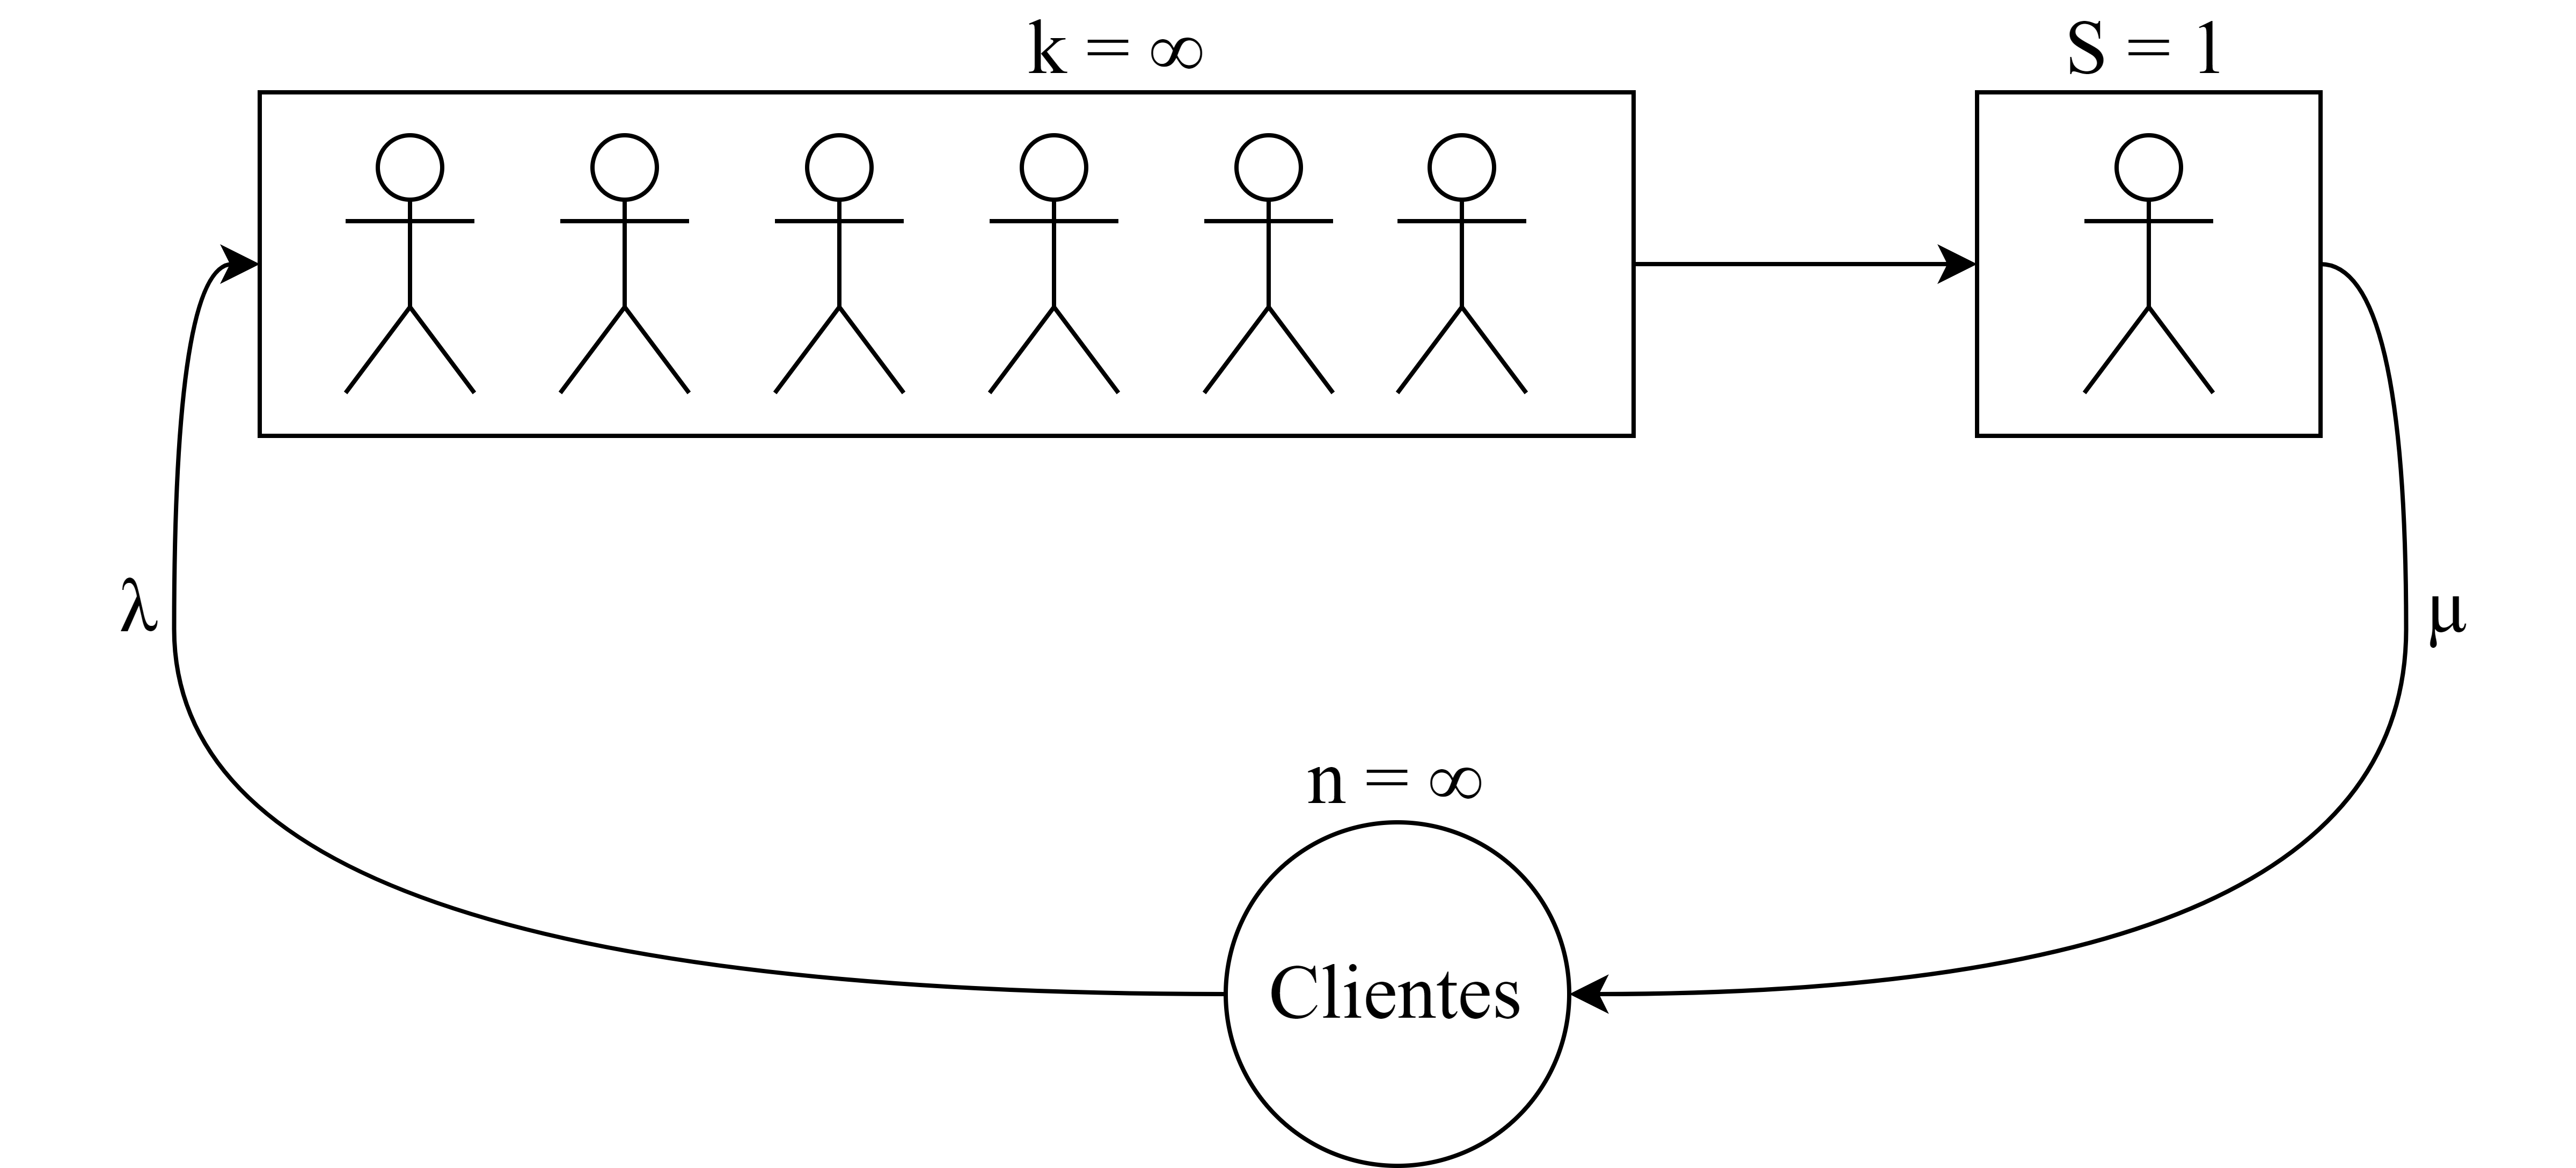
\includegraphics[width=0.8\textwidth]{img/mm1.png}
\end{figure}

\textit{Donde:}
\begin{itemize}
    \item $n$: Número de clientes en el sistema.
    \item $\lambda$: Tasa de llegada de clientes.
    \item $\mu$: Tasa de servicio.
    \item $\rho$: Factor de utilización del sistema = $\frac{\lambda}{\mu}$. \textbf{Condición de regimen:} $\rho < 1$.
\end{itemize}

\textbf{Indicadores de desempeño:}
\begin{itemize}
    \item $L$: Número promedio de clientes en el sistema = $\frac{\lambda}{\mu - \lambda}$.
    \item $L_q$: Número promedio de clientes en la cola = $\frac{\lambda^2}{\mu(\mu - \lambda)}$.
    \item $W$: Tiempo promedio de un cliente en el sistema = $\frac{1}{\mu - \lambda}$.
    \item $W_q$: Tiempo promedio de un cliente en la cola = $\frac{\lambda}{\mu(\mu - \lambda)}$.
    \item $P_0$: Probabilidad de que no haya clientes en el sistema de colas = $1 - \rho$.
    \item $P_n$: Probabilidad de que haya $n$ clientes en el sistema de colas= $(1 - \rho)\rho^n$.
    \item $P(W_q>t)$: Probabilidad de tiempo de espera en la cola = $\rho e^{-\mu(1-\rho)t}$
    \item $P(W>t)$: Probabilidad de estancia de un cliente en el sistema = $e^{-\mu(1-\rho)t}$
\end{itemize}


% \newpage
\subsection{M/M/S}
\noindent El sistema M/M/S es un sistema de colas en el que los tiempos entre llegadas y los tiempos de servicio son variables aleatorias independientes y exponenciales. En este sistema, la tasa de llegada de clientes es $\lambda$ y la tasa de servicio es $\mu$.

\begin{figure}[H]
    \centering
    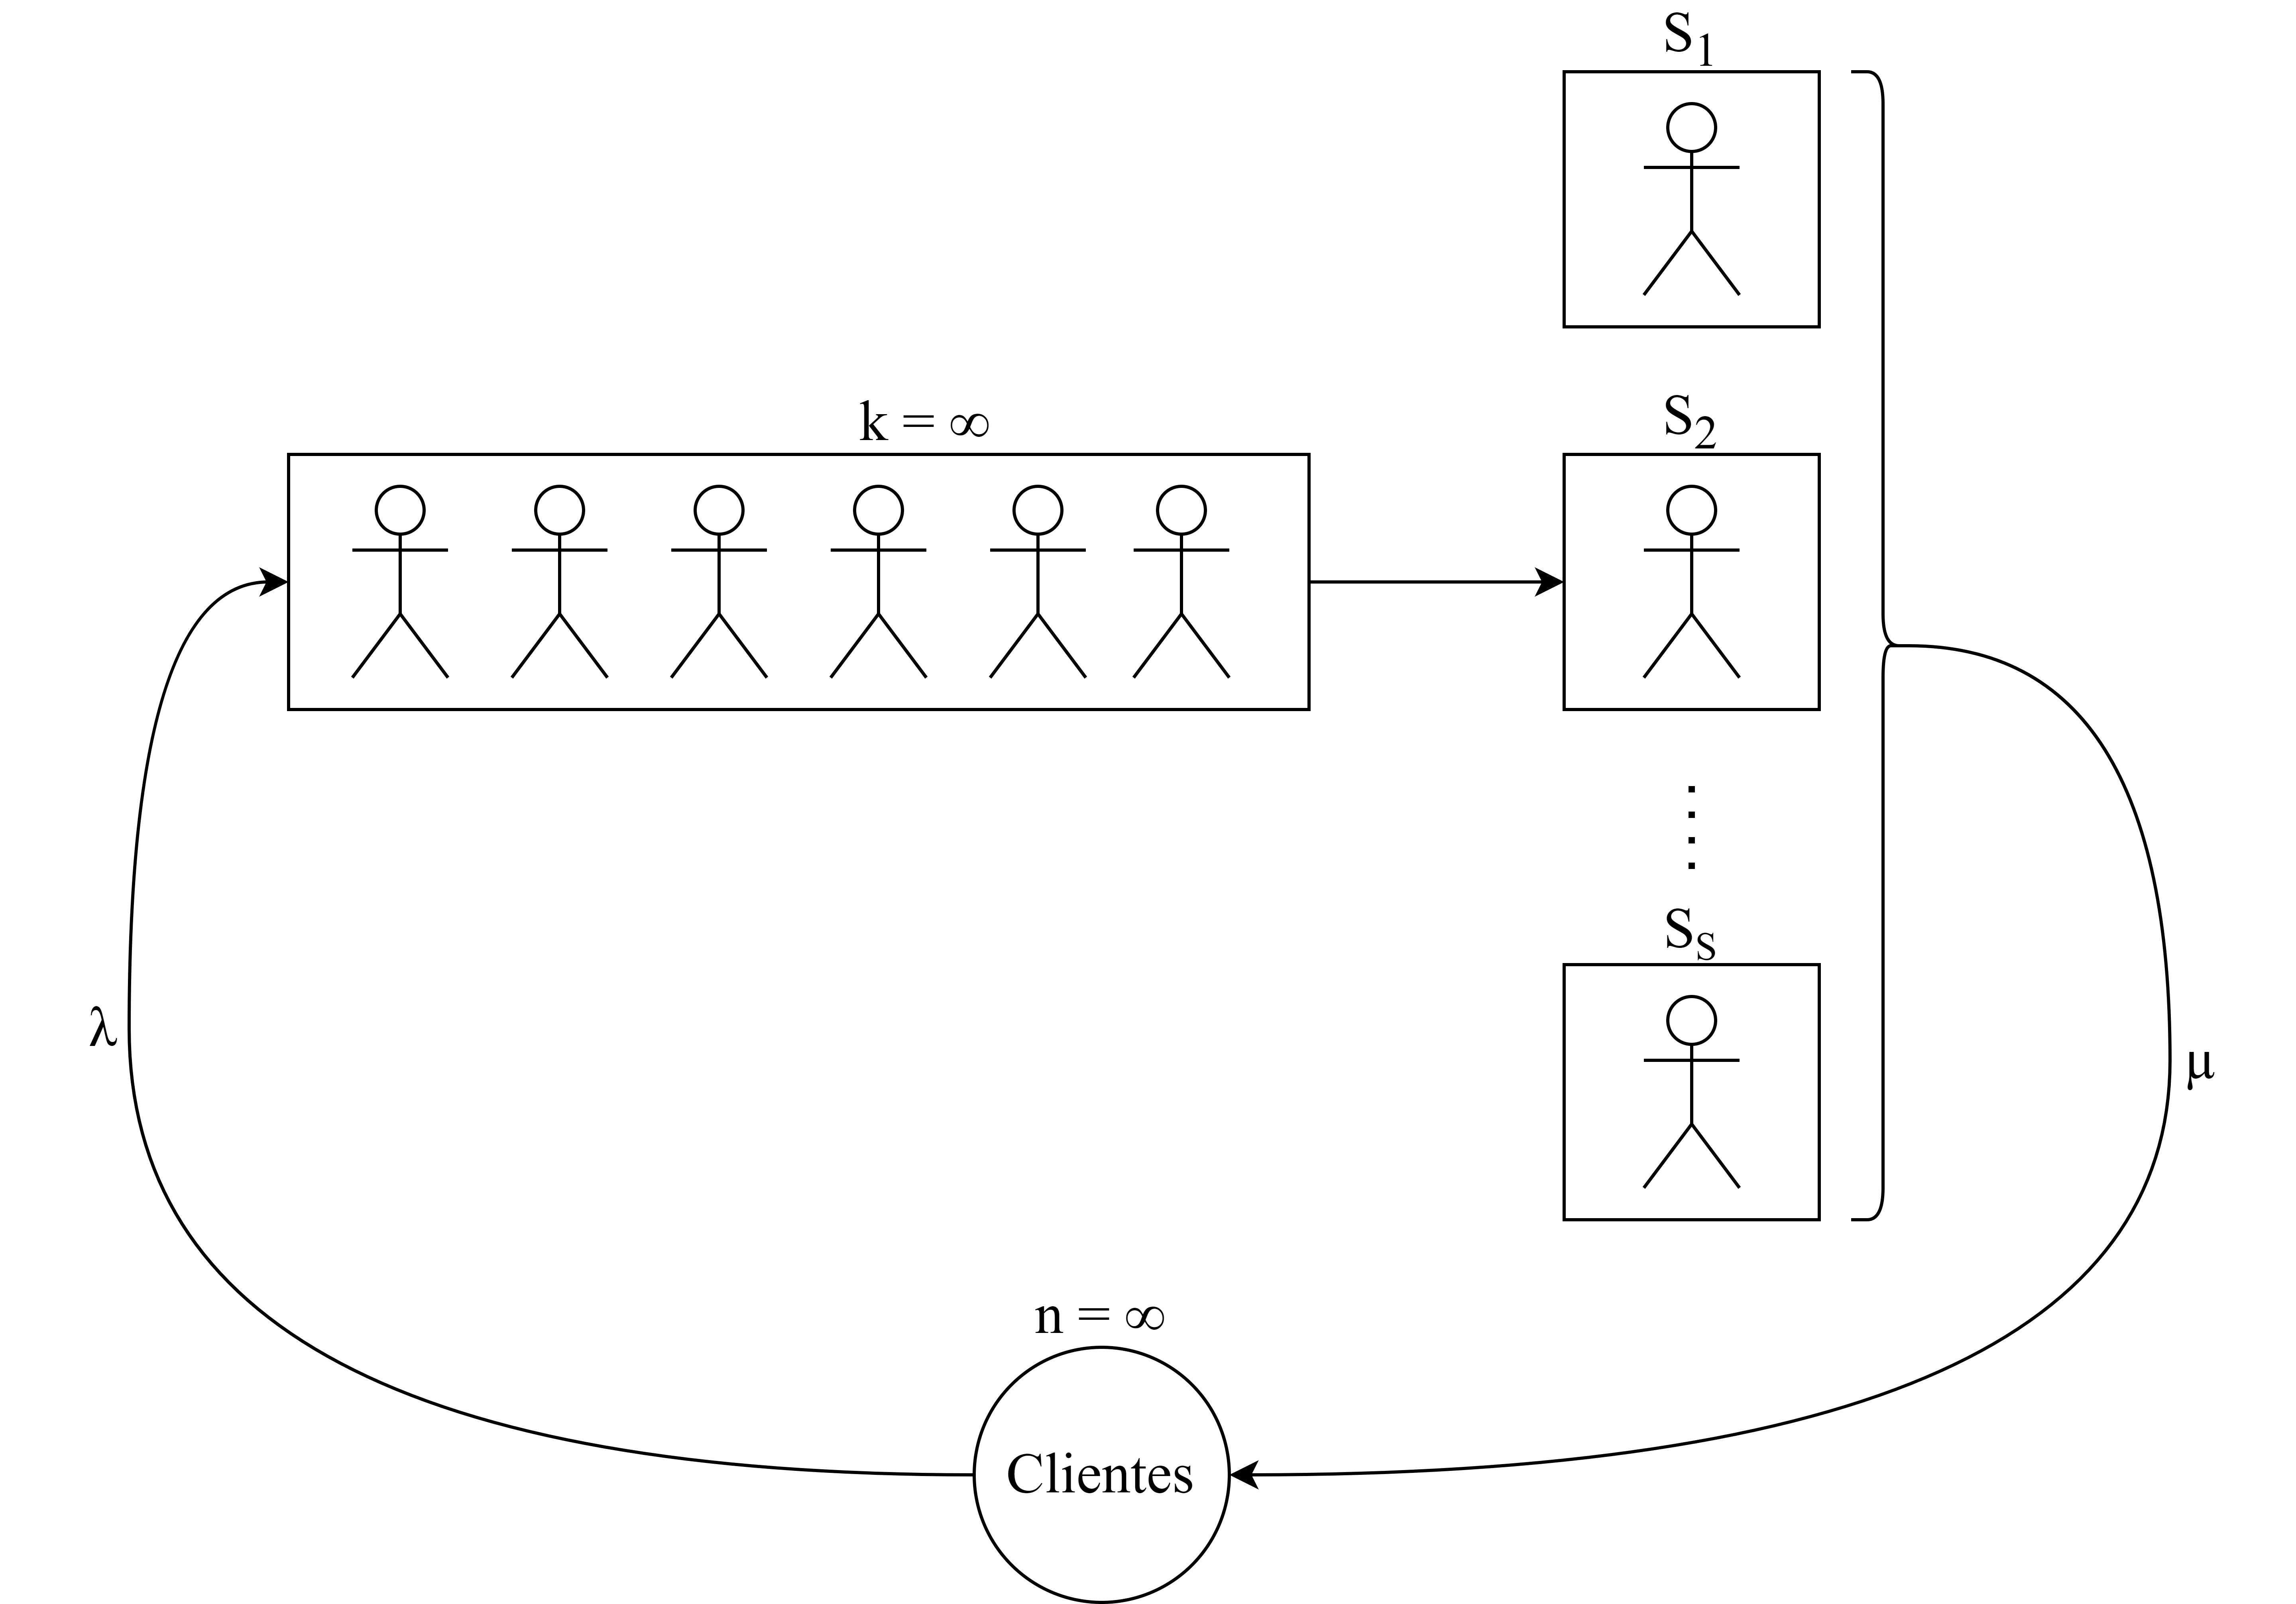
\includegraphics[width=0.8\textwidth]{img/mms.png}
\end{figure}

\textit{Donde:}
\begin{itemize}
    \item $n$: Número de clientes en el sistema.
    \item $\lambda$: Tasa de llegada de clientes.
    \item $\mu$: Tasa de servicio.
    \item $s$: Número de servidores.
    \item $\rho$: Factor de utilización del sistema = $\frac{\lambda}{S\mu}$. \textbf{Condición de regimen:} $\rho < 1$.
\end{itemize}

\textbf{Indicadores de desempeño:}
\begin{itemize}
    \item $L$: Número promedio de clientes en el sistema = $L_q + \frac{\lambda}{\mu}$ = $\lambda W_q$.
    \item $L_q$: Número promedio de clientes en la cola = $\frac{(\frac{\lambda}{\mu})^s \lambda \mu}{(s-1)! (s\mu-\lambda)^2}P_0$ = $\frac{1}{s!}(\frac{\lambda}{\mu})^s \frac{\rho}{(1-\rho)^2}P_0$.
    \item $W$: Tiempo promedio de un cliente en el sistema = $W_q+\frac{1}{\mu}$ = $\frac{L}{\lambda}$.
    \item $W_q$: Tiempo promedio de un cliente en la cola = $\frac{L_q}{\lambda}$ = $\lambda W_q$.
    \item $P_0$: Probabilidad de que no haya clientes en el sistema de colas.
    \begin{center}
        $P_0$ = $\frac{1}{\sum_{n=0}^{s-1} \frac{(\frac{\lambda}{\mu})^n}{n!} + \frac{(\frac{\lambda}{\mu})^s}{s!} (\frac{s\mu}{s\mu-\lambda})}$.
    \end{center}
    \item $P_n$: Probabilidad de que haya $n$ clientes en el sistema de colas.
    \[
    P_n = \left\{
        \begin{array}{ll}
          \frac{(\frac{\lambda}{\mu})^n}{n!}P_0 & \text{si } n \leq  s \\\\
          \frac{(\frac{\lambda}{\mu})^n}{s!}P_0 & \text{si } n > s
        \end{array}
      \right.
    \]  
    
\end{itemize}

\subsection{M/M/1/K}
\noindent El sistema M/M/1/K es un sistema de colas en el que los tiempos entre llegadas y los tiempos de servicio son variables aleatorias independientes y exponenciales. En este sistema, la tasa de llegada de clientes es $\lambda$ y la tasa de servicio es $\mu$.

\begin{figure}[H]
    \centering
    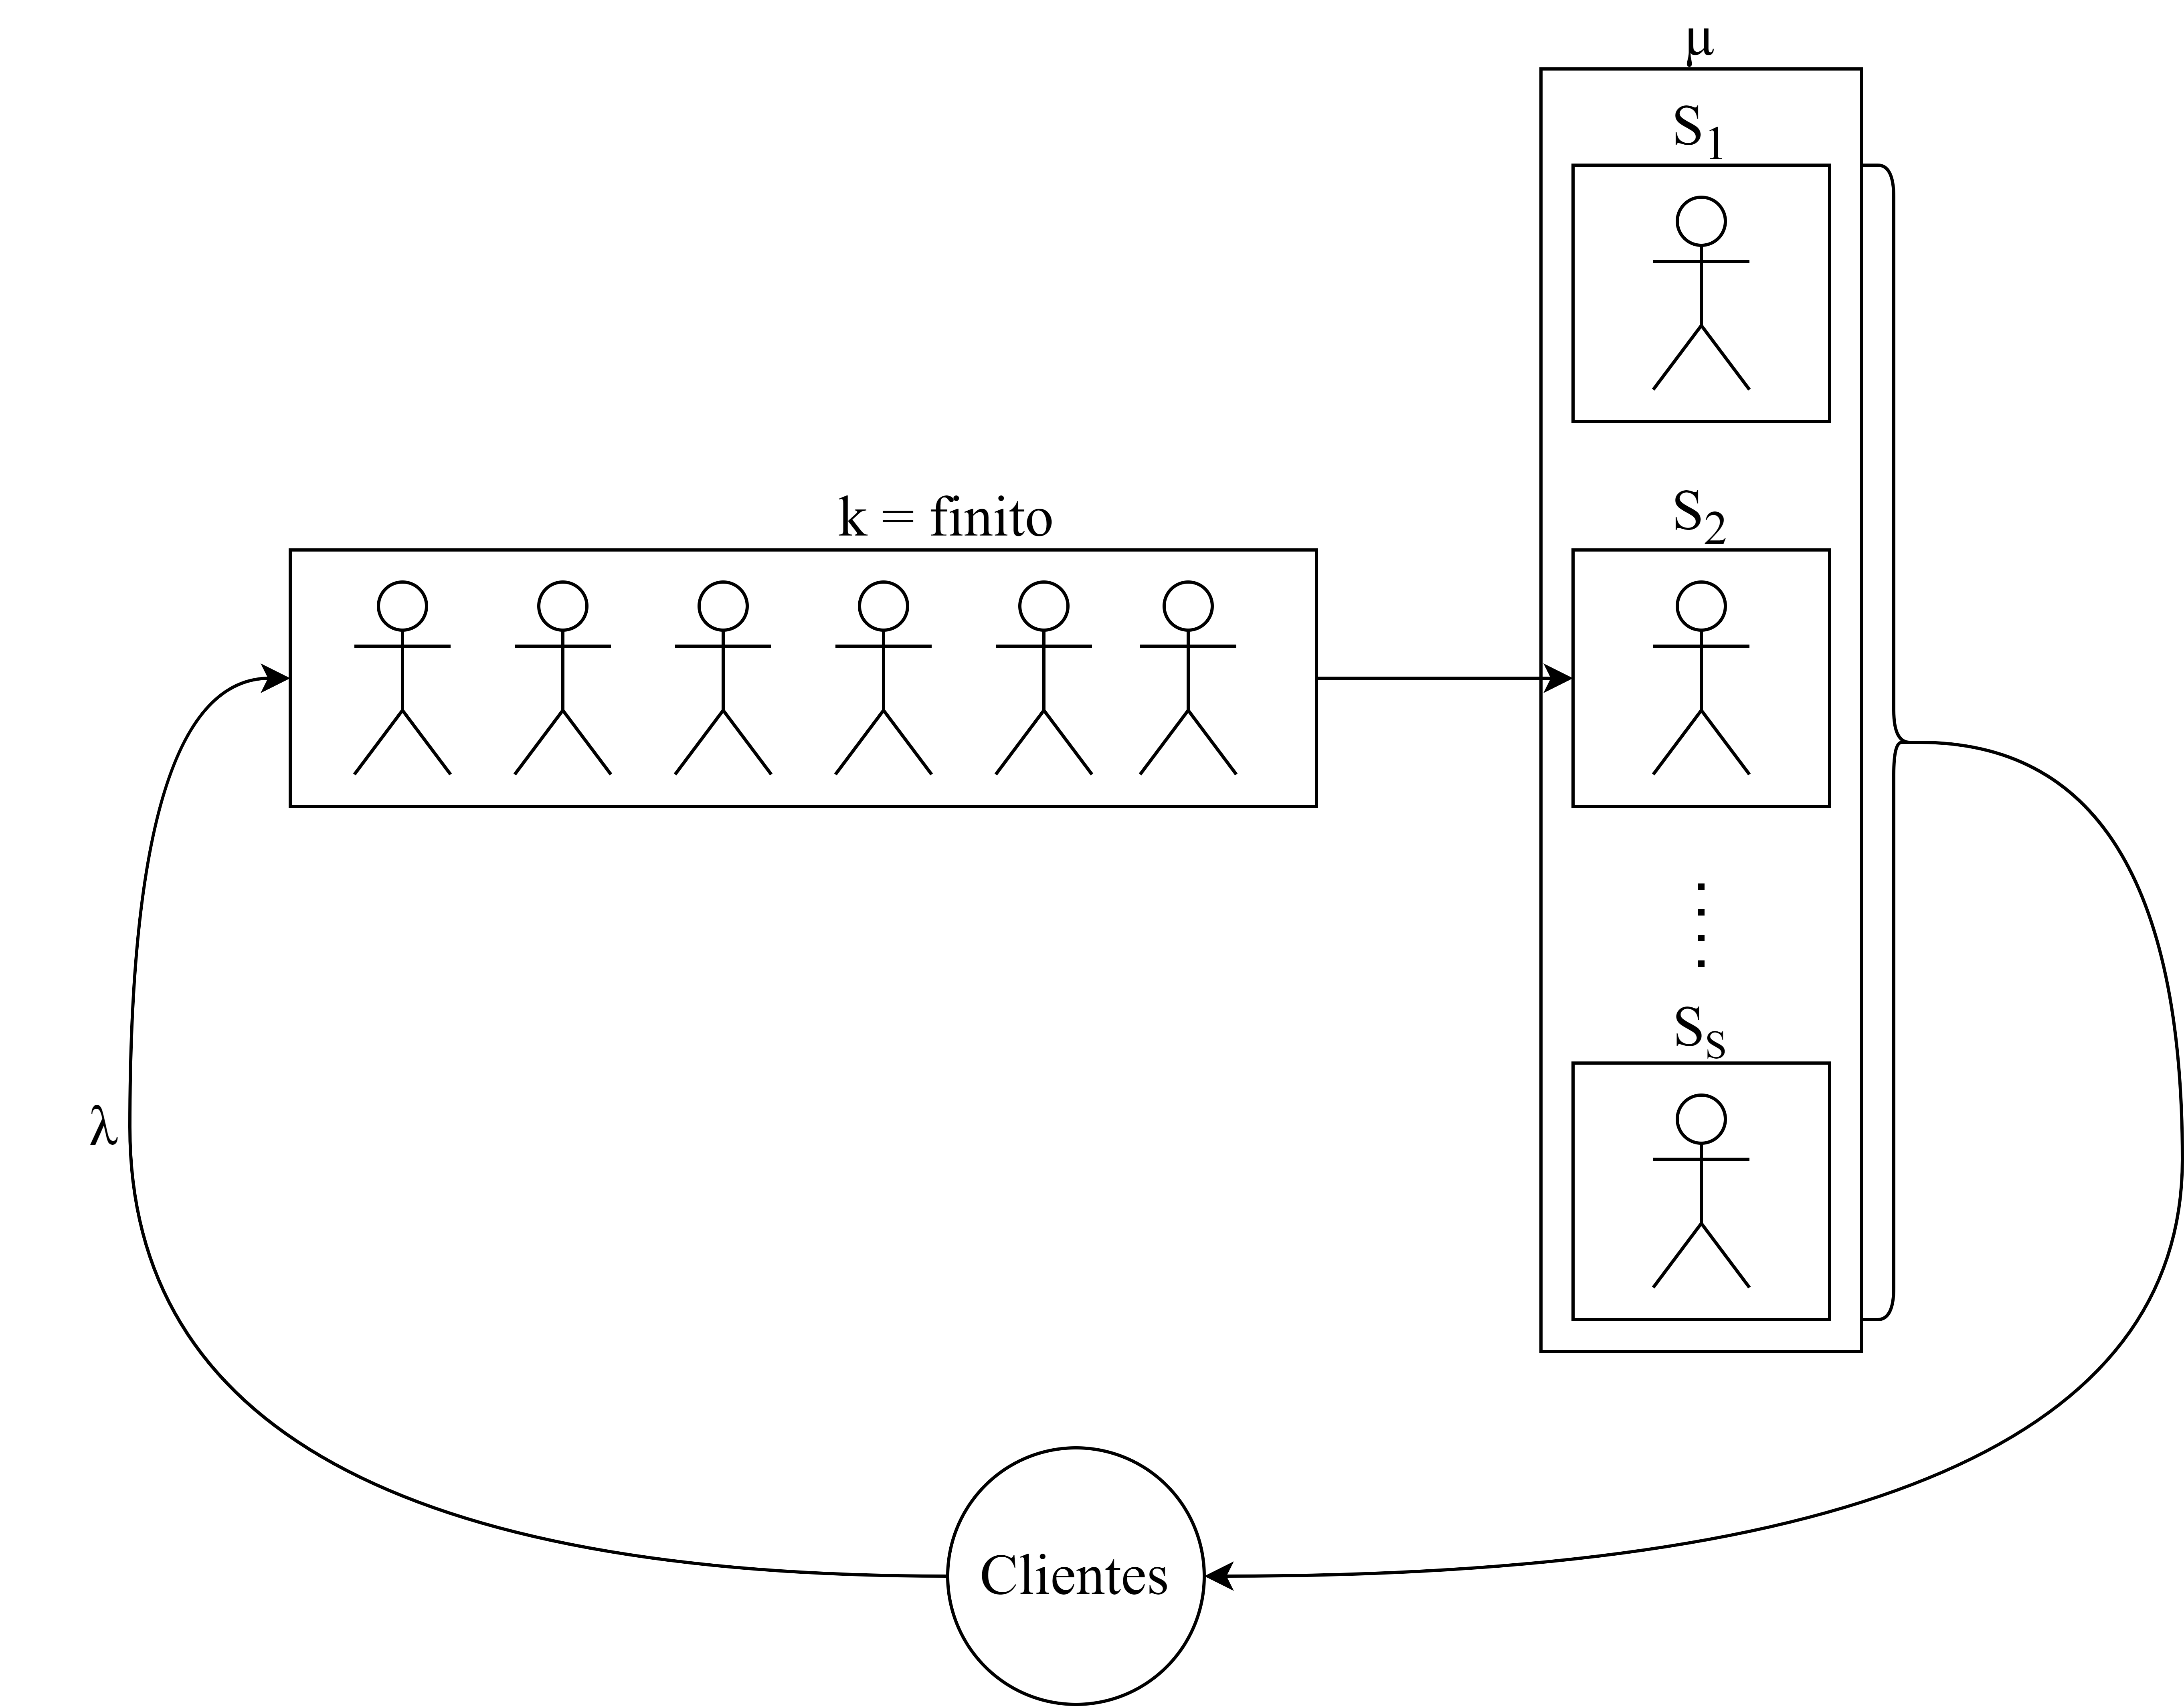
\includegraphics[width=0.8\textwidth]{img/mm1k.png}
\end{figure}

\textit{Donde:}
\begin{itemize}
    \item $n$: Número de clientes en el sistema.
    \item $\lambda$: Tasa de llegada de clientes.
    \item $\lambda_{ef}$: Tasa de llegada efectiva de clientes = $\lambda(1-P_k)$.
    \begin{itemize}
        \item \textbf{Rebote:} $\lambda - \lambda_{ef}$. 
        \item \textbf{Tasa de ingreso real al sistema:} $\lambda_{ef}<\lambda$.
    \end{itemize}
    \item $\mu$: Tasa de servicio.
    \item $K$: Capacidad del sistema.
    \item $\rho$: Factor de utilización del sistema = $\frac{\lambda}{\mu}$. \textbf{Condición de regimen:} $\rho < 1$.
\end{itemize}

\textbf{Indicadores de desempeño:}
\begin{itemize}
    \item $L$: Número promedio de clientes en el sistema.
    \[
    L = \left\{
        \begin{array}{ll}
        \frac{\rho}{1-\rho} - \frac{(k+1)\rho^{k+1}}{\rho - \rho^{k+1}} &    \text{si } \rho \neq 1 \\\\
        \frac{k}{2} &                                                        \text{si } \rho = 1
        \end{array}
      \right.
    \]  
    \item $L_q$: Número promedio de clientes en la cola.
    \[
    L_q = \left\{
        \begin{array}{ll}
        L - \frac{(1-\rho^k)\rho}{1-\rho^{k+1}} &    \text{si } \rho \neq 1 \\\\
        \frac{k(k-1)}{2(k+1)} &                        \text{si } \rho = 1
        \end{array}
      \right.
    \]
    \item $W$: Tiempo promedio de un cliente en el sistema = $\frac{L}{\lambda_{ef}}$.
    \item $W_q$: Tiempo promedio de un cliente en la cola = $\frac{L_q}{\lambda_{ef}}$.
    \item $P_0$: Probabilidad de que no haya clientes en el sistema de colas.
    \[
    P_0 = \left\{
        \begin{array}{ll}
        \frac{1-\rho}{1-\rho^{k+1}} &    \text{si } \lambda \neq \mu \equiv \rho = (\frac{\lambda}{\mu}) \neq 1  \\\\
        \frac{1}{1+k} &                  \text{si } \lambda = \mu \equiv \rho = (\frac{\lambda}{\mu}) = 1
        \end{array}
      \right.
    \]
    \item $P_n$: Probabilidad de que haya $n$ clientes en el sistema de colas.
    \[
    P_n = \left\{
        \begin{array}{ll}
        \frac{(1-\rho)\rho^n}{1-\rho^{k+1}} &    \text{si } \lambda \neq \mu \equiv \rho = (\frac{\lambda}{\mu}) \neq 1  \\\\
        \frac{1}{1+k} &                  \text{si } \lambda = \mu \equiv \rho = (\frac{\lambda}{\mu}) = 1
        \end{array}
      \right.
    \]
\end{itemize}

\subsection{Costos en sistemas de espera}
\noindent Costos atribuidos a la empresa teniendo en cuenta el tiempo de espera de los clientes en el sistema de colas y la cantidad de servidores disponibles. Se calcula a través de la siguiente fórmula:
\[
    C_t = S \cdot C_s + L \cdot C_w
\]


\newpage
\section{Formativo}
\subsection{Ejercicio 1}
\noindent A un cajero automático llegan 10 clientes por hora y cada usuario permanece en promedio 4 minutos.
\begin{enumerate}[label=(\alph*)]
    \item ¿Qué sistema es y cuáles son sus parámetros? \\
    El sistema presentado es un sistema de colas M/M/1, el cual tiene como parámetros:
    \begin{itemize}
        \item $\lambda$ = 10 $\frac{cl}{h}$
        \item \hl{$\mu$} = $\frac{60}{4} = 15 \frac{cl}{h}$ 
    \end{itemize}
    \item ¿Cuál es la tasa de utilización del cajero?
    \begin{itemize}
        \item $\rho = \frac{\lambda}{\mu} = \frac{10}{15} = 0.\overline{666}$ $\rightarrow$ $\rho < 1$ Estable
    \end{itemize}
    \item \hl{Porcentaje del tiempo que está ocupado.}
    \begin{itemize}
        \item $\%_{ocupado} = \rho \times 100 = 0.\overline{666} \times 100 = 66.\overline{6}\%$
    \end{itemize}
    \item ¿Cuántos clientes se encuentran esperando para usar el cajero en un momento dado?
    \begin{itemize}
        \item $L_q$ = $\frac{10^2}{15(15-10)}$ = $\frac{4}{3}$ = $1.\overline{3}$
    \end{itemize}
    \item ¿Cuánto tiempo utiliza un usuario en toda la operación, desde el instante inicial?
    \begin{itemize} 
        \item $W$ = $\frac{1}{\mu - \lambda}$ = $\frac{1}{15-10}$ = $\frac{1}{5}$ = 0.2 horas = 12 minutos   
    \end{itemize}
\end{enumerate}

\newpage
\subsection{Ejercicio 2}
\noindent Una ventanilla de ventas de pasajes dispone de dos personas que atienden a clientes que llega a una tasa de 80 clientes por hora. Cada vendedor es capaz de para atender a 50 clientes por hora. Se pide:
\begin{enumerate}[label=(\alph*)]
    \item Identifique el sistema y sus parámetros. \\
    El sistema presentado es un sistema de colas M/M/S de 2 servidores, con parámetros:
    \begin{itemize}
        \item $\lambda = 80 \frac{cl}{h}$
        \item $\mu = 50 \frac{cl}{h}$
        \item $s = 2$
    \end{itemize}
    \item \hl{¿Es estable el sistema?} \\
    Para conocer la estabilidad del sistema es necesario calcular el valor de la taza de utilización y si este valor es menor a 1, el sistema es estable.
    \begin{itemize}
        \item $\rho = \frac{80}{2 \cdot 50} = 0.8 < 1$
    \end{itemize}
    Por lo tanto el sistema es estable.
    \item ¿Cuál es la probabilidad que el sistema este vacío?
    \begin{align*}
        P_0 &= \frac{1}{\sum_{n=0}^{2-1} \frac{(\frac{80}{50})^n}{n!} + \frac{(\frac{80}{50})^2}{2!} \left(\frac{2\cdot50}{2\cdot50-80}\right)} \\
        &= \frac{1}{\sum_{n=0}^{1} \frac{(\frac{80}{50})^n}{n!} + \frac{(\frac{80}{50})^2}{2!} \left(\frac{2\cdot50}{2\cdot50-80}\right)} \\
        &= \frac{1}{\frac{1}{0!} + \frac{(\frac{80}{50})^1}{1!} + \frac{(\frac{80}{50})^2}{2!} \left(\frac{2\cdot50}{2\cdot50-80}\right)} \\
        &= \frac{1}{1 + \frac{80}{50} + \frac{80^2}{50^2 \cdot 2} \left(\frac{100}{20}\right)} \\
        &= \frac{1}{9} \\
        &= 0.\overline{1}
    \end{align*} 
    \item \hl{El número esperado de clientes.}\\
    
    \begin{align*}
        L &= L_q + \frac{\lambda}{\mu} \\
        &= \frac{1}{2!} (\frac{80}{50})^2 \frac{\frac{80}{100}}{(1-\frac{80}{100})^2} \cdot \frac{1}{9} + \frac{80}{50} \\
        &= \frac{1}{2!}\frac{64}{25}\cdot20\cdot\frac{1}{9} + \frac{8}{5} \\
        &= \frac{256}{45\cdot2} + \frac{8}{5} \\
        &= \frac{128}{45} + \frac{8}{5} \\
        &= \frac{40}{9}\\
        &= 4.\overline{4}
    \end{align*}
    Por lo tanto el número esperado de clientes es de 4.4.
    \item La probabilidad que haya más de 4 clientes en el sistema.
        \begin{flalign*}
        & P(n>4) = 1 - P(n\leq4) = 1 - (P_0 + P_1 + P_2 + P_3 + P_4) &\\
        &= 1 - (0.0061 + [\frac{(\frac{80}{50})^1}{1!}\cdot0.0061] + [\frac{(0.8)^2}{2!}\cdot0.0061] + [\frac{(0.8)^3}{2!}\cdot0.0061] + [\frac{(0.8)^4}{2!}\cdot0.0061])&\\
        &= 1 - (0.0061 + 0.0098 + 0.0062 + 0.0031 + 0.0012) &\\
        &= 1 - 0.0264 &\\
        &= 0.9736 &\\
        &= 97.36\% &
        \end{flalign*}
    Por lo tanto la probabilidad de que haya más de 4 clientes en el sistema es de 97.36\%.
\end{enumerate}

\newpage
\subsection{Ejercicio 3}
\noindent Encontrar las medidas de desempeño para un sistema de cola M/M/1/5 con tasa de llegada 10 y tasa de servicio igual a 12. \\

\textit{Datos:}
\begin{itemize}
    \item $\lambda = 10 \frac{cl}{h}$
    \item $\lambda_{ef} = 10(1-0.1006) = 8.994$
    \item $\mu = 12 \frac{cl}{h}$
    \item $K = 5$
    \item $\rho = \frac{10}{12} = 0.8333$
\end{itemize}

\begin{mdframed}
    \begin{align*}
        P_0 &= \frac{1-\rho}{1-\rho^6} = \frac{1-0.8333}{1-0.8333^6} = 0.1667 \\
        P_n &= \frac{(1-\rho)\rho^n}{1-\rho^6} = \frac{(1-0.8333)0.8333^n}{1-0.8333^6} \\
        P_k &= \frac{(1-0.8333)0.8333^5}{1-0.8333^6} \\
        &= 0.1006
    \end{align*}
\end{mdframed}      

\begin{mdframed}
    \begin{align*}
        L &= \frac{0.8333}{(1-0.8333)} - \frac{(6)0.8333^{6}}{1-0.8333^6} \\
        &= 4.9988 - 3.02088 \\
        &= 1.97792 \\
        &\Downarrow \\
        L_q &= 1.97792 - \frac{(1-0.8333^5)0.8333}{1-0.8333^6} \\
        &= 1.97792 - 0.749392 \\
        &= 1.228528
    \end{align*}
\end{mdframed}

\newpage
\begin{mdframed}
\begin{align*}
    W &= \frac{1.97792}{8.994}\\
    &= 0.2199 \\
    &\Downarrow \\
    W_q &= \frac{1.228528}{8.994} \\
    &= 0.1366
\end{align*}
\end{mdframed}

\newpage

\subsection{Ejercicio 4}
\noindent Un banco trata de determinar cuántos cajeros debe emplear. El costo total de emplear un cajero es 90 dólares diarios y un cajero puede atender a un promedio de 60 clientes por día. Al banco llega un promedio de 50 clientes por día y los tiempos de servicio y los tiempos entre llegadas son exponenciales. Si el costo de demora por cliente y día [en el sistema] es de 20 dólares, ¿cuántos cajeros debe contratar el banco para minimizar los costos de operación?

\textit{Datos:}
\begin{itemize}
    \item $\lambda$ = 50 $\frac{cl}{d}$
    \item $\mu$ = 60 $\frac{cl}{d}$
    \item $C_s$ = 90
    \item $C_w$ = 20
\end{itemize}

\begin{table}[h]
    \centering
    \begin{tabular}{|l|c|c|c|c|c|c|c|}
    \hline
    S & $\lambda$ & $\mu$ &$\rho$ & $P_0$ & $L_q$ & $L$ & $C_t$ \\ \hline
    1  & 50 & 60 & $\frac{50}{1\cdot60} = 0.833$ Estable & 0.1667 & 4.1667 & 5 & $1(90)+5(20)$ = 190 \\
    2  & 50 & 60 & $\frac{50}{2\cdot60} = 0.416$ Estable & 0.4117 & 0.1749 & 1.0082 & $2(90)+1.0082(20)$ = 200.16 \\
    3  & 50 & 60 & $\frac{50}{3\cdot60} = 0.277$ Estable &  &  &  &  \\
    4  & 50 & 60 & $\frac{50}{4\cdot60} = 0.208$ Estable &  &  &  &  \\
    $\vdots$ & $\vdots$ & $\vdots$ & $\vdots$ & $\vdots$ & $\vdots$ & $\vdots$ & $\vdots$ \\
    \hline
    \end{tabular}
\end{table}

Por lo tanto es conveniente contratar 1 cajero para minimizar los costos de operación.

Para un S = 1:
    \begin{align*}
        P_0 &= \frac{1}{\sum_{n=0}^{s-1} \frac{(\frac{50}{60})^n}{n!} + \frac{(\frac{50}{60})^1}{1!} (\frac{1\cdot60}{1\cdot60-50})} \\
        &= \frac{1}{\sum_{n=0}^{0} \frac{(\frac{50}{60})^n}{n!} + \frac{(\frac{50}{60})^1}{1!} (\frac{1\cdot60}{1\cdot60-50})} \\
        &= \frac{1}{\frac{1}{0!} + \frac{(\frac{50}{60})^1}{1!} (\frac{1\cdot60}{1\cdot60-50})} \\
        &= \frac{1}{1 + \frac{50}{60} \cdot \frac{60}{10}} \\
        &= \frac{1}{1 + \frac{50}{10}} \\
        &= \frac{1}{6} \\
        &= 0.1667 \\
        &\Downarrow \\
        L_q &= \frac{1}{1!} (\frac{50}{60})^1 \frac{\frac{50}{60}}{(1-\frac{50}{60})^2} \cdot \frac{1}{6} \\
        &= \frac{1}{1} \cdot \frac{50}{60} \cdot 30 \cdot \frac{1}{6} \\
        &= \frac{25}{6} \\
        &= 4.1667 \\ 
        &\Downarrow \\
        L &= 4.1667 + \frac{50}{60}\\
        &= 5
    \end{align*}

    Para un s = 2:
    \begin{align*}
        P_0 &= \frac{1}{\sum_{n=0}^{1} \frac{(\frac{50}{60})^n}{n!} + \frac{(\frac{50}{60})^2}{2!} (\frac{1\cdot60}{1\cdot60-50})} \\
        &= \frac{1}{\frac{1}{0!} + \frac{(\frac{50}{60})^1}{1!} + \frac{(\frac{50}{60})^2}{2!} (\frac{2\cdot60}{2\cdot60-50})} \\
        &= \frac{1}{\frac{1}{1}+\frac{\frac{50}{60}}{1}+\frac{(\frac{50}{60})^2}{2!}\cdot\frac{2\cdot60}{120-50}} \\
        &= \frac{1}{\frac{17}{7}} \\
        &= \frac{7}{17} \\
        &= 0.4117 \\
        &\Downarrow \\
        L_q &= \frac{1}{2!} (\frac{50}{60})^2 \frac{\frac{50}{2\cdot60}}{(1-\frac{50}{2\cdot60})^2} \cdot \frac{7}{17} \\
        &= \frac{1}{2!} \cdot \frac{25}{3} \cdot \frac{5}{7} \cdot \frac{1}{17} \\
        &= \frac{125}{714} \\
        &= 0.1749 \\
        &\Downarrow \\
        L &= 0.1749 + \frac{50}{60} \\
        &= 0.1749 + 0.8333 \\
        &= 1.0082
    \end{align*}

\end{document}